\documentclass[border=10pt]{standalone}
\usepackage{luatexja-fontspec}
\usepackage{tikz}
\usetikzlibrary{positioning, arrows.meta, calc}

% ヒラギノ丸ゴシックを指定
\setmainjfont{HiraMaruProN-W4}

\begin{document}
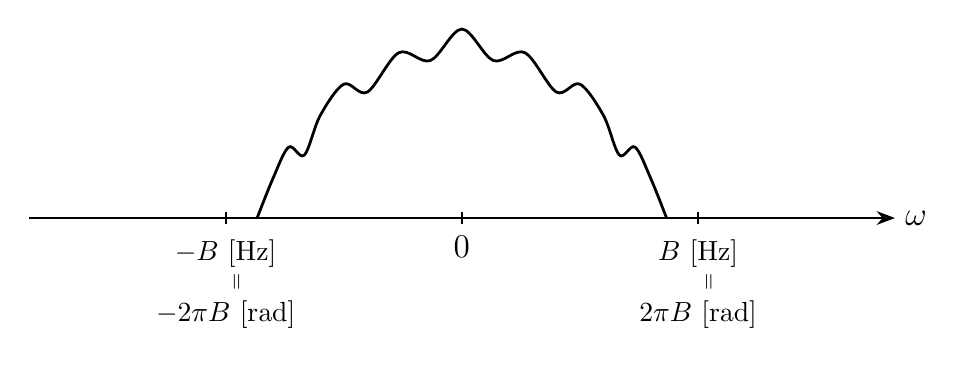
\begin{tikzpicture}[
    thick,                  % 全体の線を太めにする
    >=Stealth,              % 綺麗な矢じりを使用
    font=\large             % フォントサイズを一括で大きくする
]

    % --- 1. 座標軸の描画 ---
    % 横軸（omega軸）
    \draw [->] (-5.5, 0) -- (5.5, 0) node[right] {$\omega$};
    
    % 原点、-B、B の目盛り（小さな縦の区切り線）
    \draw (0, 0.08) -- (0, -0.08);
    \draw (-3, 0.08) -- (-3, -0.08);
    \draw (3, 0.08) -- (3, -0.08);

    % --- 2. スペクトル波形の描画（より凸凹な原点対称曲線） ---
    % 座標の点を増やし、小さな山や谷が交互に現れるよう数値を細かく調整しました
    \draw [black, line width=1.0pt, smooth, tension=0.55] plot coordinates {
        (-2.6, 0.0)
        (-2.4, 0.5)
        (-2.2, 0.9)  % 小さな肩
        (-2.0, 0.8)  % 小さなくぼみ（谷）
        (-1.8, 1.3)  % 再び立ち上がり
        (-1.5, 1.7)
        (-1.2, 1.6)  % 2番目のくぼみ
        (-0.8, 2.1)
        (-0.4, 2.0)  % 中央手前のくぼみ
        (0.0,  2.4)  % 中央の頂点
        (0.4,  2.0)  % 以下、右側へ完全ミラーリング
        (0.8,  2.1)
        (1.2,  1.6)
        (1.5,  1.7)
        (1.8,  1.3)
        (2.0,  0.8)
        (2.2,  0.9)
        (2.4,  0.5)
        (2.6,  0.0)
    };

    % --- 3. 軸下のラベル配置 ---
    % 【原点： 0】
    \node [below=0.1cm of {0, 0}] {$0$};
    
    % 【左側：-B のラベル群】
    \node [below=0.15cm of {-3, 0}, font=\normalsize] (minus_B) {$-B$ [Hz]};
    \node [below=0.05cm of minus_B, font=\normalsize, scale=0.8, rotate=90] {=};
    \node [below=0.15cm of minus_B, font=\normalsize] {$-2\pi B$ [rad]};

    % 【右側：B のラベル群】
    \node [below=0.15cm of {3, 0}, font=\normalsize] (plus_B) {$B$ [Hz]};
    \node [below=0.05cm of plus_B, font=\normalsize, scale=0.8, rotate=90] {=};
    \node [below=0.15cm of plus_B, font=\normalsize] {$2\pi B$ [rad]};

\end{tikzpicture}
\end{document}

\documentclass[border=10pt]{standalone}
\usepackage{luatexja-fontspec}
\usepackage{tikz}
\usetikzlibrary{positioning, arrows.meta, calc}

% ヒラギノ丸ゴシックを指定
\setmainjfont{HiraMaruProN-W4}

\begin{document}
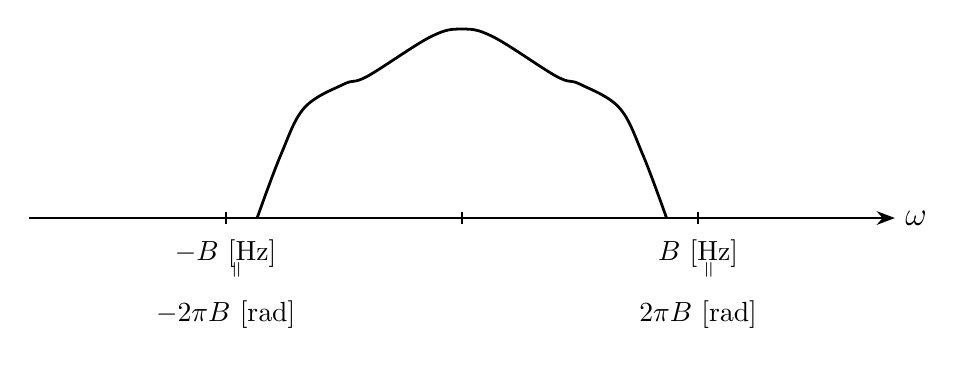
\begin{tikzpicture}[
    thick,                  % 全体の線を太めにする
    >=Stealth,              % 綺麗な矢じりを使用
    font=\large             % フォントサイズを一括で大きくする
]

    % --- 1. 座標軸の描画 ---
    % 横軸（omega軸）
    \draw [->] (-5.5, 0) -- (5.5, 0) node[right] {$\omega$};
    
    % 原点、-B、B の目盛り（小さな縦の区切り線）
    \draw (0, 0.08) -- (0, -0.08);
    \draw (-3, 0.08) -- (-3, -0.08);
    \draw (3, 0.08) -- (3, -0.08);

    % --- 2. スペクトル波形の描画（原点対称な曲線） ---
    % 手書きの凹凸感をベースに、左右の座標が完全にミラーリング（対称）になるよう設定
    \draw [black, line width=1.0pt, smooth, tension=0.6] plot coordinates {
        (-2.6, 0.0)
        (-2.3, 0.8)
        (-2.0, 1.4)
        (-1.5, 1.7)
        (-1.2, 1.8)
        (-0.4, 2.3)
        (0.0,  2.4)  % 頂点（中心）
        (0.4,  2.3)
        (1.2,  1.8)
        (1.5,  1.7)
        (2.0,  1.4)
        (2.3,  0.8)
        (2.6, 0.0)
    };

    % --- 3. 軸下のラベル配置（縦に綺麗に並べます） ---
    
    % 【左側：-B のラベル群】
    \node [below=0.15cm of {-3, 0}, font=\normalsize] (minus_B) {$-B$ [Hz]};
    \node [below=-0.1cm of minus_B, font=\normalsize, scale=0.8, rotate=90] {=};
    \node [below=0.15cm of minus_B, font=\normalsize] {$-2\pi B$ [rad]};

    % 【右側：B のラベル群】
    \node [below=0.15cm of {3, 0}, font=\normalsize] (plus_B) {$B$ [Hz]};
    \node [below=-0.1cm of plus_B, font=\normalsize, scale=0.8, rotate=90] {=};
    \node [below=0.15cm of plus_B, font=\normalsize] {$2\pi B$ [rad]};

\end{tikzpicture}
\end{document}

\documentclass[border=10pt]{standalone}
\usepackage{luatexja-fontspec}
\usepackage{tikz}
\usetikzlibrary{positioning, arrows.meta, calc}

% ヒラギノ丸ゴシックを指定
\setmainjfont{HiraMaruProN-W4}

\begin{document}
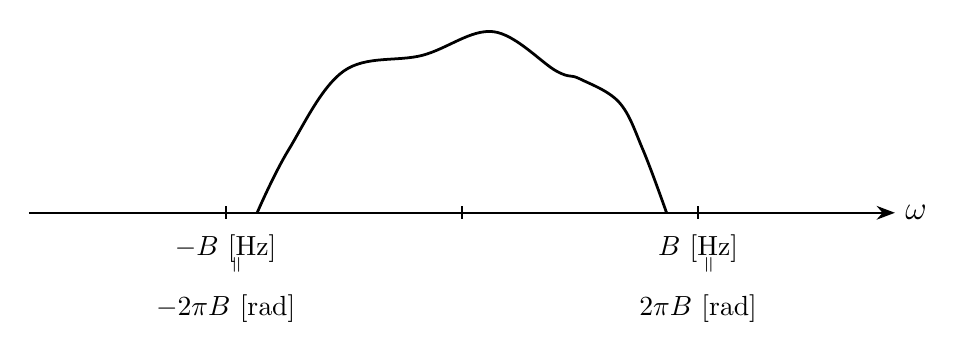
\begin{tikzpicture}[
    thick,                  % 全体の線を太めにする
    >=Stealth,              % 綺麗な矢じりを使用
    font=\large             % フォントサイズを一括で大きくする
]

    % --- 1. 座標軸の描画 ---
    % 横軸（omega軸）
    \draw [->] (-5.5, 0) -- (5.5, 0) node[right] {$\omega$};
    
    % 原点、-B、B の目盛り（小さな縦の区切り線）
    \draw (0, 0.08) -- (0, -0.08);
    \draw (-3, 0.08) -- (-3, -0.08);
    \draw (3, 0.08) -- (3, -0.08);

    % --- 2. スペクトル波形の描画（黒い滑らかな曲線） ---
    % 帯域 B（座標 3.0）未満に収まるよう、手書きの非対称な山を滑らかに表現
    \draw [black, line width=1.0pt, smooth, tension=0.6] plot coordinates {
        (-2.6, 0.0)
        (-2.2, 0.8)
        (-1.5, 1.8)
        (-0.5, 2.0)
        (0.4, 2.3)
        (1.2, 1.8)
        (1.5, 1.7)
        (2.0, 1.4)
        (2.3, 0.8)
        (2.6, 0.0)
    };

    % --- 3. 軸下のラベル配置（縦に綺麗に並べます） ---
    
    % 【左側：-B のラベル群】
    % 基準となる -B [Hz]
    \node [below=0.15cm of {-3, 0}, font=\normalsize] (minus_B) {$-B$ [Hz]};
    % 平行記号（縦向きの等号）
    \node [below=-0.1cm of minus_B, font=\normalsize, scale=0.8, rotate=90] {=};
    % 換算値 -2pi B [rad]
    \node [below=0.15cm of minus_B, font=\normalsize] {$-2\pi B$ [rad]};

    % 【右側：B のラベル群】
    % 基準となる B [Hz]
    \node [below=0.15cm of {3, 0}, font=\normalsize] (plus_B) {$B$ [Hz]};
    % 平行記号（縦向きの等号）
    \node [below=-0.1cm of plus_B, font=\normalsize, scale=0.8, rotate=90] {=};
    % 換算値 2pi B [rad]
    \node [below=0.15cm of plus_B, font=\normalsize] {$2\pi B$ [rad]};

\end{tikzpicture}
\end{document}

